\documentclass[11pt]{article}
\usepackage{amsmath,amsthm,amssymb,fullpage,graphicx,hyperref,listings}
\usepackage{listings,color,setspace}
\author{Andy Reagan}
\title{Math 337 Homework 06}

     \def\NN{\mathbb{N} }
     \def\ZZ{\mathbb{Z} }
     \def\QQ{\mathbb{Q} }
     \def\RR{\mathbb{R} }
     \def\CC{\mathbb{C} }
     \def\f{\frac }
     \def\b{\begin }
     \def\e{\end }
     \def\Log{\text{Log} \,}
     \def\Re{\text{Re} \, }

\lstset{language=MATLAB,
basicstyle=\ttfamily\scriptsize\singlespacing,
keywordstyle=\color{blue},
stringstyle=\color{red},
commentstyle=\color{green},
morecomment=[l][\color{magenta}]{\#},
frame=L,
xleftmargin=\parindent,
%%numbers=left,                   %% where to put the line-numbers
%%numberstyle=\scriptsize,      %% the size of the fonts that are used for the line-numbers
%%stepnumber=1,                   %% the step between two line-numbers. If it is 1 each line will be numbered
numbersep=5pt,
breaklines=true,        %% sets automatic line breaking
breakatwhitespace=false,    %% sets if automatic breaks should only happen at whitespace
escapeinside={\%*}{*)} 
}


     \newcommand{\pdiff}[2]{\frac{\partial #1}{\partial #2}}
     \newcommand{\partialdiff}[2]{\frac{\partial #1}{\partial #2}}
     \newcommand{\pdiffsq}[2]{\frac{\partial^2 #1}{{\partial #2}^2}}
     \newcommand{\pdiffcu}[2]{\frac{\partial^3 #1}{{\partial #2}^3}}
     \newcommand{\pdiffhi}[3]{\frac{\partial^#3 #1}{{\partial #2}^#3}}
     \newcommand{\diff}[2]{\frac{{\rm d}#1}{{\rm d}#2}}
     \newcommand{\diffsq}[2]{\frac{{\rm d}^{2}#1}{{\rm d} {#2}^2}}
     \newcommand{\diffhi}[3]{\frac{{\rm d}^#3 #1}{{\rm d} {#2}^#3}}
     \newcommand{\tdiff}[2]{\mbox{d} #1/\mbox{d} #2}
     \newcommand{\tdiffsq}[2]{\mbox{d}^{2} #1/\mbox{d} {#2}^2}
     \newcommand{\tpdiff}[2]{\partial #1/\partial #2}
     \newcommand{\tpdiffsq}[2]{\partial^2 #1/\partial {#2}^2}
     \newcommand{\bvec}[1]{\vec{ {\bf #1 } }}
     \newcommand{\oh}[1]{O(h^{{#1}})}

\begin{document}
\maketitle

\begin{enumerate}

\item Verify that the {\em homogeneous} versions of Problems I and III in the notes have nontrivial solutions, while the homogeneous version of Problem II has only the trivial solution.

\bigskip
\textbf{Solution:} The homogeneous version of Problem I is the same the homogeneous version of Problem III. This is:
\begin{align*} y'' + \pi ^2 y = 0, ~~~~y(0) = 0, ~~~~y(1) = 0. \end{align*}
From the notes, equation 6.6, we have the general solution given by 
\begin{align*} y = A \sin \pi x + B\cos \pi x. \end{align*}
For the first BC, we see that $y(0) = B = 0$.
Similarly, $y(1) = -B = 0$.
Therefore, $y = A \sin \pi x$ is a solution to the ODE and both BC, for arbitrary $A$, so there are nontrivial (infinitely many) solutions.

The homogeneous version of Problem II is:
\begin{align*} y'' + \pi ^2 y = 0, ~~~~y(0) = 0, ~~~~y'(1) = 0. \end{align*}
Again, for the first BC, we see that $y(0) = B = 0$.
For the second BC, $y'(1) = A = 0$.
Therefore, the only solution is $y(x) = 0$, the trivial solution.


\bigskip
\item Find the solution of Problem I with the $\pi ^2$ replaced by $(\pi + \epsilon)^2$, where $\epsilon << 1$.
Based on your answer, explain why such a problem is ill-posed.


\bigskip
\textbf{Solution:} We have the solution from equation 6.6 as 
\begin{align*} y = A \sin (\pi+\epsilon) x + B\cos (\pi+\epsilon) x + \f{1}{(\pi+\epsilon)^2}. \end{align*}
The first BC simply gives us that $B = -\f{1}{(\pi+\epsilon)^2}$.
The second BC is more complicated, so I write it out (using the appropriate trig identities followed by the Maclaurin series):
\begin{align*} 0 &= y(1) = A \sin (\pi+\epsilon) -\f{1}{(\pi+\epsilon)^2} \cos (\pi+\epsilon) + \f{1}{(\pi+\epsilon)^2}\\
&= -A \sin \epsilon + \f{\cos \epsilon }{(\pi+\epsilon)^2} + \f{1}{(\pi+\epsilon)^2}\\
&= -A \epsilon + \f{1 }{(\pi+\epsilon)^2} + \f{1}{(\pi+\epsilon)^2} + O(\epsilon ^3)\\
&\simeq -A \epsilon + \f{2}{(\pi+\epsilon)^2} \end{align*}
Solving this for $A$, we have
\begin{align*}A \simeq \f{2}{\epsilon (\pi+\epsilon)^2}\end{align*}
We observe here that for $\epsilon$ small, $A$ is very large, and very sensitive to the value of epsilon and behaves as $1/\epsilon$.
As $\epsilon \to 0$, we have $A \to \infty$.\\

%% Alternatively, we can write this as a linear system
%% \begin{align*}\left ( \begin{array}{cc} 0 & 1 \\ -\epsilon & 1 \end{array} \right ) \left ( \begin{array}{c} A \\ B \end{array} \right ) = \left ( \begin{array}{c} -\f{1}{(\pi+\epsilon)^2} \\ -\f{1}{(\pi+\epsilon)^2} \end{array} \right ) \end{align*}
%% The condition number of solving this system (the ratio of the singular values) is given by the eigenvalues of the LHS matrix multiplied by its transpose.
%% That is, we compute the eigenvalues of 
%% \begin{align*}\left ( \begin{array}{cc} 0 & -\epsilon  \\ 1 & 1 \end{array} \right )\left ( \begin{array}{cc} 0 & 1 \\ -\epsilon & 1 \end{array} \right ) = \left ( \begin{array}{cc} \epsilon ^2  & -\epsilon \\ -\epsilon & 2 \end{array} \right ) \end{align*}

%% \[ \lambda _{1,2} = \f{4+4\epsilon^2+\epsilon^4+\sqrt{16-32\epsilon^2+24\epsilon^4+8\epsilon^6+\epsilon^8}}{4+4\epsilon^2+\epsilon^4-\sqrt{16-32\epsilon^2+24\epsilon^4+8\epsilon^6+\epsilon^8}} \]
%% This is not very helpful, so I make a plot of this for $\epsilon \in [0,0.1]$.
%% We see the same as above, for small $\epsilon$ the condition number of the matrix explodes, making this problem ill-posed.

%% \begin{figure}[h!]
%%   \centering
%%     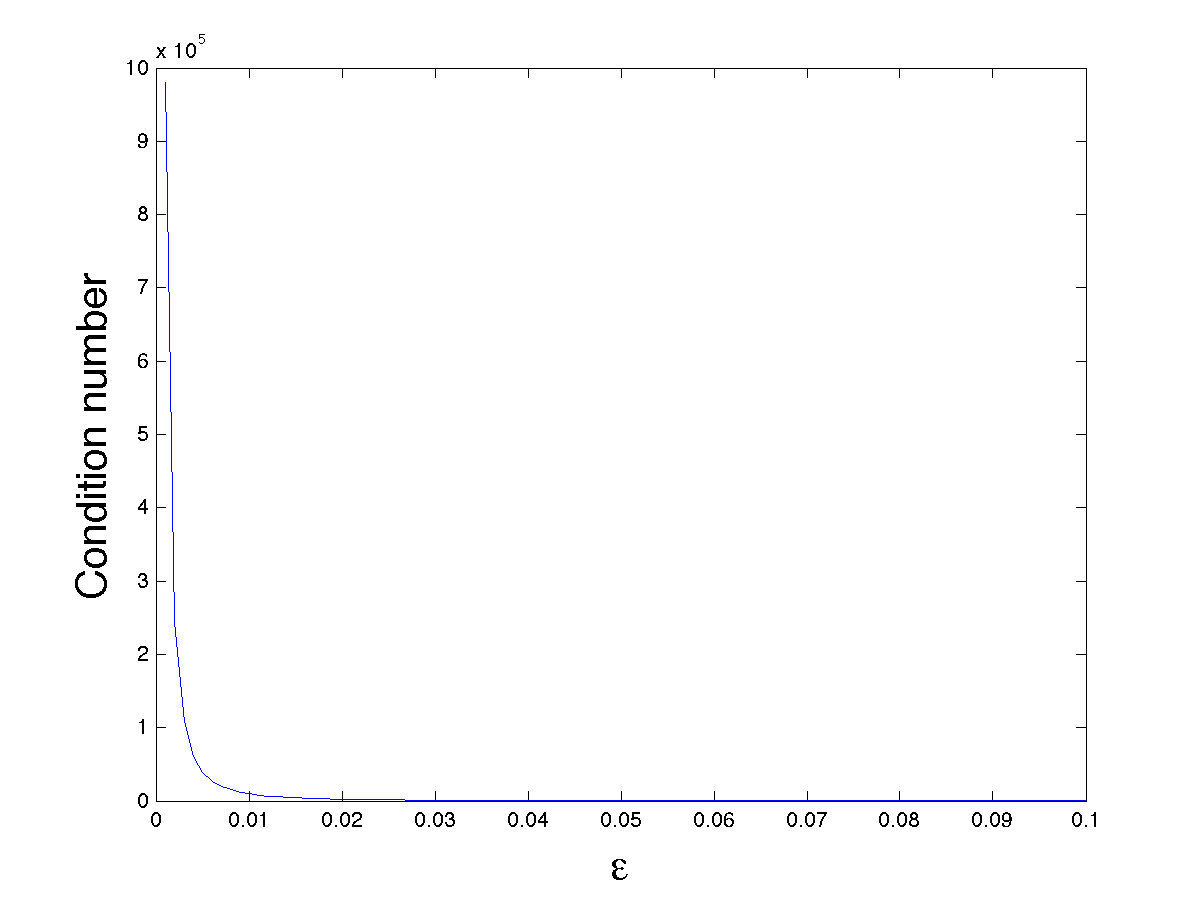
\includegraphics[width=0.5\textwidth]{andy_hw06_prb2_01.png}
%%   \caption{Condition number of the linear BVP for small $\epsilon$.}
%% \end{figure}

%% \lstinputlisting[language=Matlab]{andy_hw06_prb2.m}

\end{enumerate}

%% %% \begin{figure}[h!]
%% %%   \centering
%% %%     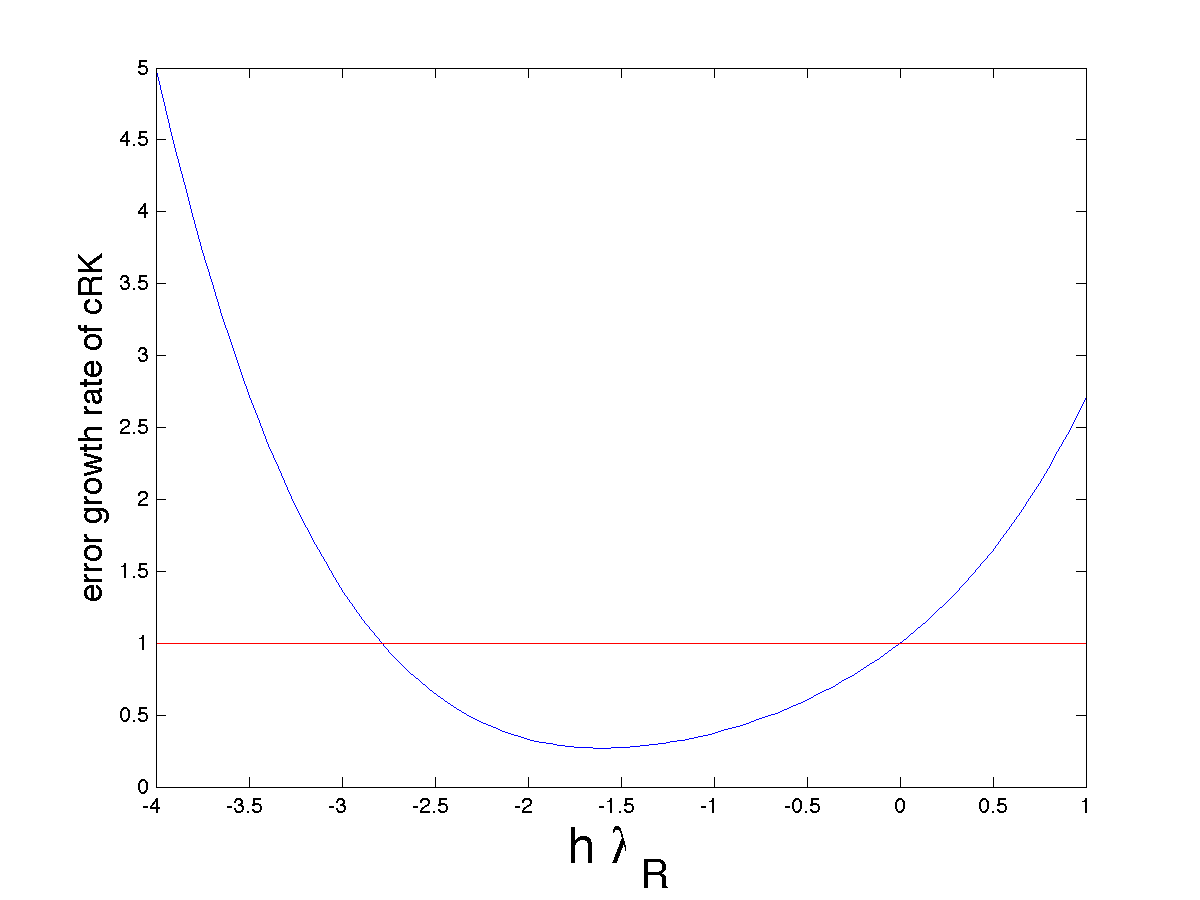
\includegraphics[width=0.5\textwidth]{andy_hw04_prb02_01.png}
%% %%   \caption{Stability of the cRK method.}
%% %% \end{figure}

%% %% \lstinputlisting[language=Matlab]{andy_hw04_prb04.m}

\end{document}


